%%%%%%%%%%%%%%%%%%%%%%%%%%%%%%%%%%%%%%%%%
% Stylish Article
% LaTeX Template
% Version 2.1 (1/10/15)
%
% This template has been downloaded from:
% http://www.LaTeXTemplates.com
%
% Original author:
% Mathias Legrand (legrand.mathias@gmail.com) 
% With extensive modifications by:
% Vel (vel@latextemplates.com)
%
% License:
% CC BY-NC-SA 3.0 (http://creativecommons.org/licenses/by-nc-sa/3.0/)
%
%%%%%%%%%%%%%%%%%%%%%%%%%%%%%%%%%%%%%%%%%

%----------------------------------------------------------------------------------------
%	PACKAGES AND OTHER DOCUMENT CONFIGURATIONS
%----------------------------------------------------------------------------------------

\documentclass[fleqn,10pt]{SelfArx} % Document font size and equations flushed left

\usepackage[english]{babel} % Specify a different language here - english by default

\graphicspath{ {./img/} }

\usepackage{float}

\usepackage[export]{adjustbox}

%----------------------------------------------------------------------------------------
%	COLUMNS
%----------------------------------------------------------------------------------------

\setlength{\columnsep}{0.55cm} % Distance between the two columns of text
\setlength{\fboxrule}{0.75pt} % Width of the border around the abstract

%----------------------------------------------------------------------------------------
%	COLORS
%----------------------------------------------------------------------------------------

\definecolor{color1}{RGB}{0,0,90} % Color of the article title and sections
\definecolor{color2}{RGB}{200,200,200} % Color of the boxes behind the abstract and headings
\definecolor{color3}{RGB}{200,200,200}

%----------------------------------------------------------------------------------------
%	HYPERLINKS
%----------------------------------------------------------------------------------------

\usepackage{hyperref} % Required for hyperlinks
\hypersetup{hidelinks,colorlinks,breaklinks=true,urlcolor=color1,citecolor=color1,linkcolor=color1,bookmarksopen=false,pdftitle={Title},pdfauthor={Author}}

%----------------------------------------------------------------------------------------
%	ARTICLE INFORMATION
%----------------------------------------------------------------------------------------

\JournalInfo{Introduction to Data Analysis  and Mining 2022} % Journal information
\Archive{} % Additional notes (e.g. copyright, DOI, review/research article)

\PaperTitle{Semester Project} % Article title

\Authors{Joshua Elms\textsuperscript{1}*} % Authors
\affiliation{\textsuperscript{1}\textit{Computer Science, School of Informatics , Computing and Engineering, Indiana University, Bloomington, IN, USA}} % Author affiliation


\Keywords{Meteorology --- Numerical Weather Prediction --- Machine Learning} % Keywords - if you don't want any simply remove all the text between the curly brackets
\newcommand{\keywordname}{Keywords} % Defines the keywords heading name

%----------------------------------------------------------------------------------------
%	ABSTRACT
%----------------------------------------------------------------------------------------

\Abstract{This data analytics project is focused on predicting the size of largest hailstone that comes from any given storm. To do this, reports of more than 20,000 hail events and their associated meteorological data have been collected and tabularized.}

%----------------------------------------------------------------------------------------

\begin{document}

\flushbottom % Makes all text pages the same height

\maketitle % Print the title and abstract box

\tableofcontents % Print the contents section

\thispagestyle{empty} % Removes page numbering from the first page




%----------------------------------------------------------------------------------------
%Problem and Data Description
%----------------------------------------------------------------------------------------


\section{Problem and Data Description} % The \section*{} command stops section numbering

\:According to the NOAA Annual Severe Weather website, there were 3,762 recorded severe hail events (hail over 0.75") in the US in 2021 alone. Beyond the noble goal of furthering our understanding of the natural world, the ability to accurately predict which locations will experience hail storms could benefit insurance companies who pay out an average of \$12,000 for residential damage claims and \$4,000 for automobile claims. Multiplied by thousands of storms per year and hundreds of thousands of possible claims per storm, it is clear that increasing advanced warming times for likely hail conditions could have massive benefits for both the general public and insurance companies alike.

The data for this project consists of approximately 29,000 reports of severe hail events and the meteorological conditions present during the event. The hail event data was collected from the 2012-2016 entries in the \href{https://www.spc.noaa.gov/wcm/#data}{NOAA Storm Prediction Center database}. After extracting just the hail sizes, coordinates, and dates/times, those parameters were entered into the North American Mesoscale Model to determine vertical profiles of temperature, humidity, and wind within 3 hours and 20 km of the individual hail events. The meteorological profiles were passed to an open-source python program, \href{https://github.com/sharppy/SHARPpy}{SHARPpy}, to calculate the exclusively continuous, numerical parameters we will be discussing in the following table.

After the data is extracted from the various sources and tabularized, it forms a CSV with 21902 entries and 55 fields, including the target variable of hailstone size.
\begin{figure}[H]
\centering
\includegraphics[width = 4.5cm, height = 15cm]{"table2.png"}
\end{figure}

\bigskip
\bigskip

%----------------------------------------------------------------------------------------
%	Data Preprocessing $\&$ Exploratory Data Analysis
%----------------------------------------------------------------------------------------

\section{Data Preprocessing $\&$ Exploratory Analysis} % The \section*{} command stops section numbering

\subsection{Parameter Selection}
After the pipeline detailed in the Data Description was traversed, there were 53 parameters associated with each severe hail event (not including Hail Size). The 11 of the parameters (index positions 1-10 and 27) were repeated three times throughout the data, with the only difference being slightly different calculation methods for each. The three methods used were SB (Surface Based), ML (Mixed Layer), and MU (Most Unstable), each of which describes a process for calculating thermodynamic and wind related parameters. In short, SB uses the temperature at the surface, ML uses an average of the conditions up to an altitude of 100 mb (millibars), and MU uses the temperature of the most unstable air parcel found in the lowest 300 mb of the atmosphere. For a more in-depth explanation, refer to the \href{https://www.spc.noaa.gov/exper/mesoanalysis/help/begin.html}{NOAA Storm Prediction Center's guide} on the subject.

We first attempted to determine how well these these various calculation techniques track each other by generating correlation plots corresponding to each of the first 10 variables. It our hope that they would all perform almost identically and thereby allow only one set to be used for visualization, analysis, and modeling purposes. However, the chart makes it clear that this is not the case.

\begin{figure}[H]
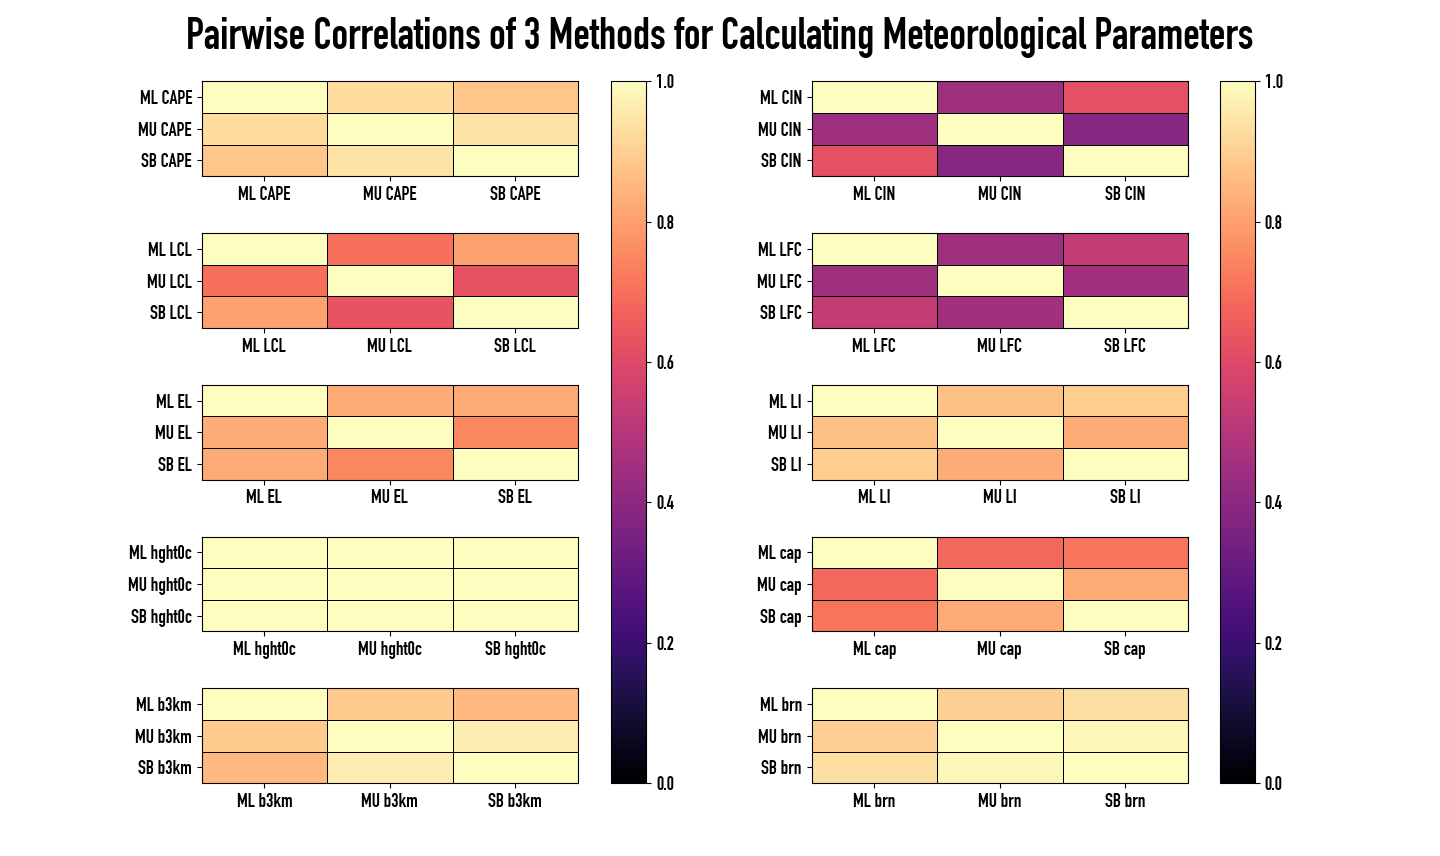
\includegraphics[width=1.15\textwidth, right=19cm]{"plots/big_corrplot.png"} 
\end{figure}

I include more text here for the purpose of... uh... testing. I include more text here for the purpose of... uh... testing. I include more text here for the purpose of... uh... testing. I include more text here for the purpose of... uh... testing.I include more text here for the purpose of... uh... testing. I include more text here for the purpose of... uh... testing. I include more text here for the purpose of... uh... testing. I include more text here for the purpose of... uh... testing.I include more text here for the purpose of... uh... testing. I include more text here for the purpose of... uh... testing. I include more text here for the purpose of... uh... testing. I include more text here for the purpose of... uh... testing.I include more text here for the purpose of... uh... testing. I include more text here for the purpose of... uh... testing. I include more text here for the purpose of... uh... testing. I include more text here for the purpose of... uh... testing.

I include more text here for the purpose of... uh... testing. I include more text here for the purpose of... uh... testing. I include more text here for the purpose of... uh... testing. I include more text here for the purpose of... uh... testing.I include more text here for the purpose of... uh... testing. I include more text here for the purpose of... uh... testing. I include more text here for the purpose of... uh... testing. I include more text here for the purpose of... uh... testing.

\clearpage

\subsection{Handling Missing Values}

\subsection{Exploratory Data Analysis}


\bigskip
\bigskip
%----------------------------------------------------------------------------------------
 % Algorithm and Methodology
%----------------------------------------------------------------------------------------


\section{Algorithm and Methodology}

Briefly explain the algorithms in this section, i.e., linear regressions. You can add more subsections if needed, i.e., regression trees etc.


\bigskip
\bigskip
%----------------------------------------------------------------------------------------
 % Experiments and Results
%----------------------------------------------------------------------------------------
\section{Experiments and Results}


\bigskip
\bigskip
%----------------------------------------------------------------------------------------
 % Summary and Conclusions
%----------------------------------------------------------------------------------------
\section{Summary and Conclusions}
\bigskip
\bigskip
\bigskip



\phantomsection
\section*{Acknowledgments} % The \section*{} command stops section numbering

\addcontentsline{toc}{section}{Acknowledgments} % Adds this section to the table of contents



%----------------------------------------------------------------------------------------
%	REFERENCE LIST
%----------------------------------------------------------------------------------------
\phantomsection
\bibliographystyle{unsrt}
\bibliography{sample}

%----------------------------------------------------------------------------------------

\end{document}